\documentclass[tikz,border=2pt]{standalone}
\usepackage{tikz}
\usepackage{tikz}
\usepackage{lmodern}
\usetikzlibrary{calc,decorations.pathreplacing}

% Visual conventions follow the existing MRNC TikZ pictures: ordinary
% components use TikZ's normal 0.4pt stroke, with compact TeX labels.
\tikzset{
  nu fibre/.style={
    x=0.78cm,
    y=0.78cm,
    line width=0.4pt,
    line cap=round,
    line join=round
  },
  nu label/.style={
    font=\scriptsize,
    inner sep=1pt
  },
  nu annotation/.style={
    font=\scriptsize,
    inner sep=1pt
  },
  nu dots/.style={
    font=\small,
    inner sep=0pt
  }
}

\begin{document}

% IV-II_l (l >0)
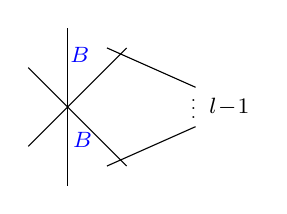
\begin{tikzpicture}[scale=0.5]
  % Coordinates
  \coordinate (A) at (-3.00, 4.00);
  \coordinate (B) at (-3.00, 0.00);
  \coordinate (E) at (-4.00, 1.00);
  \coordinate (F) at (-1.50, 3.50);
  \coordinate (C) at (-4.00, 3.00);
  \coordinate (D) at (-1.50, 0.50);
  \coordinate (G) at (-2.00, 3.50);
  \coordinate (H) at (0.25, 2.50);
  \coordinate (I) at (-2.00, 0.50);
  \coordinate (J) at (0.25, 1.50);
  \coordinate (K) at (0.2, 1.5);
  \coordinate (K_1) at (1.11, 1.53);
  \coordinate (G_1) at (-2.69, 2.89);
  \coordinate (L) at (-2.62, 0.73);

  % Drawing
  \draw (A) -- (B);
  \draw (E) -- (F);
  \draw (C) -- (D);
  \draw (G) -- (H);
  \draw (I) -- (J);
  \node[scale=0.8, font=\fontsize{8.5}{9}\selectfont][above] at (K) {$\vdots$};
  \node[font=\fontsize{8.5}{9}\selectfont][above] at (K_1) {$l\!-\!1$};
  \node[above, text=blue, font=\fontsize{8.5}{9}\selectfont] at (G_1) {$B$};
  \node[above, text=blue, font=\fontsize{8.5}{9}\selectfont] at (L) {$B$};
\end{tikzpicture}

\end{document}
